\documentclass[aspectratio=169,10pt]{beamer}
\usetheme{Madrid}
\usecolortheme{default}
\usepackage{tikz}
\usepackage{booktabs}
\usepackage{fontawesome5}
\usepackage{xcolor}
\usepackage{amsmath}
\usepackage{colortbl}
\usetikzlibrary{arrows.meta,shadows,positioning,fit,shapes.geometric,calc}

% ── palette ──────────────────────────────────────────────────────────
\definecolor{c1}{RGB}{41,128,185}
\definecolor{c2}{RGB}{52,152,219}
\definecolor{c3}{RGB}{155,89,182}
\definecolor{c4}{RGB}{142,68,173}
\definecolor{c5}{RGB}{230,126,34}
\definecolor{c6}{RGB}{211,84,0}
\definecolor{hit}{RGB}{39,174,96}
\definecolor{miss}{RGB}{192,57,43}
\definecolor{warn}{RGB}{243,156,18}

\setbeamercolor{frametitle}{bg=c1,fg=white}
\setbeamercolor{title}{fg=white}
\setbeamercolor{structure}{fg=c1}
\setbeamertemplate{navigation symbols}{}
\setbeamertemplate{footline}[frame number]
\setbeamerfont{frametitle}{series=\bfseries}

\newcommand{\chit}[1]{\cellcolor{hit!30} #1}
\newcommand{\cmiss}[1]{\cellcolor{miss!25} #1}
\newcommand{\cwarn}[1]{\cellcolor{warn!30} #1}
\newcommand{\czero}{\cellcolor{black!4} }

\title{\textbf{Graph-Based Vulnerability Retrieval}\\[4pt]}
\subtitle{Master's Thesis — Technical Progress · Checkpoint 3}
\author{Lívia}
\institute{TU Munich · Siemens}
\date{\today}


\begin{document}

% ── title ─────────────────────────────────────────────────────────────
\begin{frame}
\titlepage
\end{frame}

% ── agenda ────────────────────────────────────────────────────────────
\begin{frame}{Agenda}
  \begin{enumerate}
    \item[\textcolor{c1}{\faIcon{redo}}]
      \textbf{Checkpoint 2 recap} — results \& open questions

    \vspace{0.45em}
    \item[\textcolor{c6}{\faIcon{cut}}]
      \textbf{Slicing ablation} — full graph vs.\ sliced, with/without diff labels

    \vspace{0.45em}
    \item[\textcolor{c3}{\faIcon{sitemap}}]
      \textbf{CWE ontology} — structure \& Wu-Palmer similarity

    \vspace{0.45em}
    \item[\textcolor{c2}{\faIcon{code-branch}}]
      \textbf{Cross-CVE callgraph} — shared callee signatures as a second signal

    \vspace{0.45em}
    \item[\textcolor{c4}{\faIcon{sort-amount-up}}]
      \textbf{Knowledge-augmented reranking} — embedding $+$ Jaccard fusion

    \vspace{0.45em}
    \item[\textcolor{c5}{\faIcon{layer-group}}]
      \textbf{Embedder ensembles} — majority vote, cascade, RRF strategies

    \vspace{0.45em}
    \item[\textcolor{miss}{\faIcon{th}}]
      \textbf{Confusion analysis} — where every embedder still fails

    \vspace{0.45em}
    \item[\textcolor{hit}{\faIcon{lightbulb}}]
      \textbf{Key findings \& next steps}
  \end{enumerate}
\end{frame}

% ══════════════════════════════════════════════════════════════════════
\section{Recap}
% ══════════════════════════════════════════════════════════════════════

\begin{frame}{Checkpoint 2 Recap: Results}
\begin{columns}[T]
\begin{column}{0.50\textwidth}
  \textbf{Dataset \& setup}
  \begin{itemize}
    \item 225 pairs (75 original CVEs + LLM re-implementations)
    \item Semantic fingerprint diff $\rightarrow$ $G_{\text{vuln}}$ subgraph
    \item 8 embedders; HNSW index; self-retrieval \& CWE recall
  \end{itemize}

  \vspace{0.9em}
  \textbf{Best results (self-retrieval, $n=225$)}

  \vspace{0.3em}
  {\small
  \renewcommand{\arraystretch}{1.25}
  \begin{tabular}{lcc}
    \toprule
    \textbf{Embedder} & \textbf{SR@1} & \textbf{CWE Recall} \\
    \midrule
    \rowcolor{c1!10}
    Combined (NetLSD+WL+GIN) & 86.3\% & 51.9\% \\
    GIN                      & 75.3\% & 39.8\% \\
    CodeBERT seq             & 75.3\% & 41.2\% \\
    NetLSD                   & 32.9\% & 21.0\% \\
    \bottomrule
  \end{tabular}}
\end{column}
\begin{column}{0.47\textwidth}
  \centering
  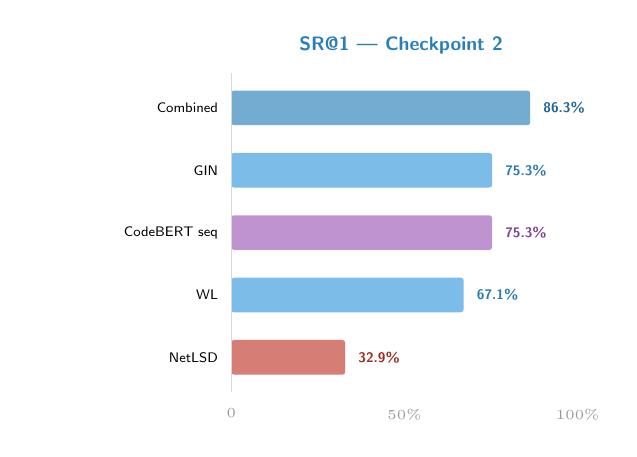
\begin{tikzpicture}[scale=0.88]
    \foreach \y/\lbl/\col/\val/\pct in {
      4.5/{Combined}/c1/0.863/86.3\%,
      3.6/{GIN}/c2/0.753/75.3\%,
      2.7/{CodeBERT seq}/c3/0.753/75.3\%,
      1.8/{WL}/c2/0.671/67.1\%,
      0.9/{NetLSD}/miss/0.329/32.9\%}{
      \node[left,font=\tiny\sffamily,text width=2.3cm,align=right] at (0,\y) {\lbl};
      \fill[\col!65,rounded corners=1pt]
        (0.05,\y-0.25) rectangle ({0.05+5.0*\val},\y+0.25);
      \node[right,font=\tiny\sffamily\bfseries,\col!80!black]
        at ({0.05+5.0*\val+0.05},\y) {\pct};
    }
    \draw[black!15] (0.05,0.4)--(0.05,5.0);
    \node[below,font=\tiny\color{black!40}] at (0.05,0.3) {0};
    \node[below,font=\tiny\color{black!40}] at (2.55,0.3) {50\%};
    \node[below,font=\tiny\color{black!40}] at (5.05,0.3) {100\%};
    \node[font=\scriptsize\sffamily\bfseries,c1] at (2.5,5.4) {SR@1 — Checkpoint 2};
  \end{tikzpicture}
\end{column}
\end{columns}
\end{frame}

\begin{frame}{Checkpoint 2 Recap: Open Questions}
  \begin{enumerate}
    \item[\faIcon{question-circle}]
      \textbf{Can the CWE ontology help post-rank results?}\\
      Errors were semantically coherent — NullPtr retrieved as UAF.
      Can the taxonomy assign a soft penalty to taxonomically far misses?

    \vspace{0.8em}
    \item[\faIcon{question-circle}]
      \textbf{Do shared function calls carry discriminative signal?}\\
      Deadlock patches call locking primitives; UAF patches call
      allocation/free functions. Is callee overlap enough to build
      a second similarity score?

    \vspace{0.8em}
    \item[\faIcon{question-circle}]
      \textbf{Does ensembling multiple embedders help?}\\
      Structural and semantic embedders fail on different queries.
      Combining them should recover at least some cases.

    \vspace{0.8em}
    \item[\faIcon{question-circle}]
      \textbf{How honest are our numbers?}\\
      Self-retrieval is circular — augmented variants share callees and
      graph structure with their originals.
      A held-out set is needed before drawing strong conclusions.
  \end{enumerate}
\end{frame}

% ══════════════════════════════════════════════════════════════════════
\section{Slicing Ablation}
% ══════════════════════════════════════════════════════════════════════

\begin{frame}{Slicing Ablation: Nomenclature \& Metrics}
\begin{columns}[T]
\begin{column}{0.50\textwidth}

  \textbf{Graph variants}

  \vspace{0.3em}
  {\small
  \renewcommand{\arraystretch}{1.4}
  \begin{tabular}{p{2.5cm}p{4.5cm}}
    \toprule
    \textbf{Symbol} & \textbf{Definition} \\
    \midrule
    $G_{\text{before}}$
      & Full pre-patch CPG.  No diff labels, no slicing. \\
    $G_{\text{before}}^{+\ell}$
      & Full pre-patch CPG $+$ diff labels transferred from $G_{\text{vuln}}$.
        Same size, extra node annotations. \\
    $G_{\text{vuln}}^{-\ell}$
      & Fingerprint-sliced subgraph.  Diff attributes (\texttt{diff}, \texttt{diff\_weight}) stripped. \\
    $G_{\text{vuln}}$
      & Fingerprint-sliced subgraph $+$ diff labels $+$ weights
        ($w \in \{1.0, 0.8, 0.6, 0.2\}$). \\
    \bottomrule
  \end{tabular}}

  \vspace{0.6em}
  {\scriptsize\color{black!55}
  Labels: \texttt{removed} ($w{=}1.0$), \texttt{fix\_adjacent} ($w{=}0.8$),
  \texttt{edge\_changed} ($w{=}0.6$), \texttt{context} ($w{=}0.2$).}

\end{column}
\begin{column}{0.47\textwidth}

  \textbf{Evaluation metrics}

  \vspace{0.3em}
  {\small
  \renewcommand{\arraystretch}{1.35}
  \begin{tabular}{p{2.0cm}p{4.5cm}}
    \toprule
    \textbf{Metric} & \textbf{Definition} \\
    \midrule
    hit@$k$
      & Fraction of queries whose correct CVE appears in top-$k$ results. \\
    MRR
      & Mean reciprocal rank of the first correct CVE. \\
    CVE Prec.
      & Per-CVE binary hit (was the CVE found in top-$k$?), macro-averaged across CVE classes. \\
    CVE Recall
      & Fraction of same-CVE index items retrieved in top-$k$, macro-averaged. \\
    CWE Recall
      & Fraction of same-CWE items retrieved, macro-averaged over CWE classes. \\
    \bottomrule
  \end{tabular}}

  \vspace{0.3em}
  {\scriptsize\color{black!55}
  All precision/recall/F1 are \textbf{macro-averaged} per class
  (each CVE/CWE contributes equally regardless of frequency).}

\end{column}
\end{columns}
\end{frame}

\begin{frame}{Slicing Ablation: Three Experiment Configurations}

  {\small\textbf{All runs:} 225 index, 73 query (seed=42, stratified).}

  \vspace{0.3em}
  {\scriptsize
  \renewcommand{\arraystretch}{1.35}
  \begin{tabular}{p{1.0cm}p{2.8cm}p{2.7cm}p{2.5cm}p{3.5cm}}
    \toprule
    & \textbf{Run A} & \textbf{Run B} & \textbf{Run C} \\
    & {\scriptsize\texttt{ade634}} & {\scriptsize\texttt{e27850}} & {\scriptsize\texttt{f7fa6a}} \\
    \midrule
    \textbf{Script}
      & \texttt{slicing\_comparison}
      & \texttt{slicing\_comparison}
      & \texttt{runner.py} \\
    \textbf{Query protocol}
      & Symmetric (query = same variant as index)
      & \texttt{runner\_compat} (augmented$\to G_{\text{before}}$,\newline original$\to G_{\text{vuln}}$)
      & Same as Run~B (implemented natively) \\
    \textbf{PCA}
      & Reset per variant; fit on index $\cup$ query batch
      & Reset per variant; fit on index $\cup$ query batch
      & Fit on index only; query projected through index PCA \\
    \textbf{Embed}
      & \texttt{embed\_many} (batch)
      & \texttt{embed\_many} (batch)
      & \texttt{embed\_one} per query \\
    \bottomrule
  \end{tabular}}

  \vspace{0.3em}
  \begin{alertblock}{PCA leakage in Runs A \& B}
    \scriptsize \texttt{slicing\_comparison.py} resets PCA per variant and calls \texttt{embed\_many()}
    on index+query together $\Rightarrow$ PCA fitted on query data too (information leakage).
    Run~C follows correct IR protocol: PCA fitted on index only, queries projected through it.
  \end{alertblock}

\end{frame}


\begin{frame}{Slicing Ablation: Results — $G_{\text{vuln}}$ (hit@1, $n{=}73$)}

  \vspace{-0.4em}
  {\scriptsize
  \renewcommand{\arraystretch}{1.2}
  \setlength{\tabcolsep}{4pt}
  \begin{tabular}{l *{3}{c} c *{3}{c} c *{3}{c}}
    \toprule
    & \multicolumn{3}{c}{\textbf{Run A} {\scriptsize(symmetric, PCA leak)}}
    && \multicolumn{3}{c}{\textbf{Run B} {\scriptsize(runner\_compat, PCA leak)}}
    && \multicolumn{3}{c}{\textbf{Run C} {\scriptsize(runner\_compat, correct PCA)}} \\
    \cmidrule{2-4} \cmidrule{6-8} \cmidrule{10-12}
    \textbf{Embedder}
      & hit@1 & MRR & CWE
      && hit@1 & MRR & CWE
      && hit@1 & MRR & CWE \\
    \midrule
    \rowcolor{c1!12}
    Combined
      & 73.9\% & .776 & .429
      && \chit{90.4\%} & \chit{.925} & \chit{.543}
      && 82.2\% & .881 & .527 \\
    GIN
      & 69.9\% & .742 & .411
      && 73.9\% & .788 & .450
      && 72.6\% & .773 & .408 \\
    CodeBERT seq
      & \chit{76.7\%} & .796 & .395
      && 75.3\% & .792 & .412
      && 75.3\% & .793 & .412 \\
    CodeBERT pat.
      & \chit{76.7\%} & .792 & .409
      && 71.2\% & .768 & .414
      && 71.2\% & .768 & .415 \\
    WL
      & 67.1\% & .711 & .365
      && 67.1\% & .720 & .432
      && 65.8\% & .702 & .415 \\
    RGCN
      & 53.4\% & .629 & .339
      && 60.3\% & .676 & .372
      && 60.3\% & .676 & .372 \\
    \bottomrule
  \end{tabular}}

  \vspace{0.3em}
  \begin{columns}[T]
  \begin{column}{0.48\textwidth}
    {\scriptsize\textbf{Key observations}}
    \begin{itemize}\setlength{\itemsep}{1pt}
      {\scriptsize
      \item Combined is the \textbf{best embedder in every run}
      \item Run B inflates Combined by $+$8.2~pp vs.\ Run C (PCA leakage)
      \item CodeBERT seq stable across all runs ($\approx$75\%)}
    \end{itemize}
  \end{column}
  \begin{column}{0.48\textwidth}
    {\scriptsize\textbf{CodeBERT is PCA-insensitive}}
    \begin{itemize}\setlength{\itemsep}{1pt}
      {\scriptsize
      \item CodeBERT seq/pattern: nearly identical in Runs B \& C
      \item High intrinsic dim (768d) makes PCA less impactful}
    \end{itemize}
  \end{column}
  \end{columns}
\end{frame}


\begin{frame}{Combined Embedder: Why the Performance Varies}
\begin{columns}[T]
\begin{column}{0.52\textwidth}

  \textbf{Combined = NetLSD $\|$ WL $\|$ GIN $\to$ PCA $\to$ L2}\\[3pt]
  {\small Three structural sub-embedders concatenated (384d),
  PCA-projected to 128d, L2-normalised.}

  \vspace{0.5em}
  \textbf{Why PCA leakage inflates Combined most}
  \begin{enumerate}\setlength{\itemsep}{3pt}
    {\small
    \item \textbf{High raw dimensionality} (384d) makes PCA
          the dominant transformation — small changes in
          the covariance matrix shift all projections.
    \item \textbf{Query graphs are structurally similar to
          index graphs} (augmented variants share topology).
          Including them in PCA fitting aligns the projection
          axes to maximise variance across both sets.
    \item For CodeBERT (768d $\to$ 128d), the first 128 PCA
          components already capture $>95$\% of variance —
          adding queries barely shifts the subspace.}
  \end{enumerate}

\end{column}
\begin{column}{0.45\textwidth}

  \textbf{Effective dimensionality confirms this}

  \vspace{0.4em}
  {\small
  \renewcommand{\arraystretch}{1.3}
  \begin{tabular}{lcc}
    \toprule
    \textbf{Embedder} & \textbf{Run B} & \textbf{Run C} \\
    & {\scriptsize PCA leak} & {\scriptsize correct} \\
    \midrule
    \rowcolor{c1!10}
    Combined         & \textbf{32.5} & 10.4 \\
    CodeBERT seq     & 15.3 & 14.7 \\
    CodeBERT pat.    & 16.8 & 15.4 \\
    GIN              & 10.0 & 11.0 \\
    WL               & 8.0 & 4.6 \\
    RGCN             & 2.3 & 2.0 \\
    \bottomrule
  \end{tabular}}

  \vspace{0.5em}
  {\scriptsize\color{black!55}
  With PCA leakage, Combined's effective dim triples
  (10.4 $\to$ 32.5), meaning the projection captures
  more discriminative directions — but at the cost of
  fitting to test data.}

  \vspace{0.4em}
  {\scriptsize\color{black!55}
  Run C (82.2\%) is the trustworthy number for Combined.}

\end{column}
\end{columns}
\end{frame}


\begin{frame}{Structural vs.\ Semantic Embedders: Analysis}
\begin{columns}[T]
\begin{column}{0.50\textwidth}

  \textbf{Structural embedders} {\small(GIN, WL, Combined)}

  \vspace{0.2em}
  \begin{itemize}\setlength{\itemsep}{2pt}
    {\scriptsize
    \item Operate on \textbf{graph topology + node types} only — no pretrained LM.
    \item \textbf{Combined is best overall} (82.2\% hit@1, Run C) — three complementary views
          (spectrum, colour refinement, message passing).
    \item GIN alone: 72.6\% — message-passing on node types is moderately discriminative.
    \item WL (65.8\%) — low effective dim (4.6), colour histogram loses information.
    \item \textbf{Strength:} fast ($<$10s for 225 graphs), no model dependencies.
    \item \textbf{Weakness:} blind to code semantics — topologically identical patches
          with different variable names $\to$ same embedding.}
  \end{itemize}

\end{column}
\begin{column}{0.47\textwidth}

  \textbf{Semantic embedders} {\small(CodeBERT seq, CodeBERT pat.)}

  \vspace{0.2em}
  \begin{itemize}\setlength{\itemsep}{2pt}
    {\scriptsize
    \item \textbf{CodeBERT [CLS]} on changed code text.
          Pattern variant adds 34 structural features.
    \item \textbf{Remarkably stable}: CodeBERT seq $\approx$ 75\% in every run —
          insensitive to PCA protocol, variant, and query strategy.
    \item Diff labels: modest $+$1.4~pp boost (\texttt{diff\_weight} $> 0.3$ filter).
    \item \textbf{Strength:} captures code semantics (variable names, API calls, strings).
    \item \textbf{Weakness:} ignores graph connectivity (seq); pattern adds $+$0~pp in Run C.}
  \end{itemize}

  \vspace{0.3em}
  \begin{block}{\scriptsize Conclusion}
    \scriptsize Graph structure carries \textbf{more discriminative signal}
    than code text for vulnerability retrieval.
    Combined (structural) beats CodeBERT by 7~pp.
    Best path forward: hybrid approach.
  \end{block}

\end{column}
\end{columns}
\end{frame}

% ══════════════════════════════════════════════════════════════════════
\section{Embedding Pipeline Ablation}
% ══════════════════════════════════════════════════════════════════════

\begin{frame}[fragile]{Embedding Pipeline: Where PCA \& L2 Normalization Sit}

  \centering
  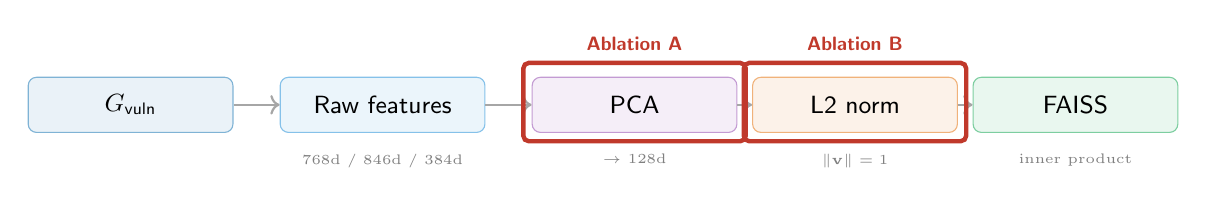
\begin{tikzpicture}[
    box/.style={rounded corners=3pt, draw=#1!60, fill=#1!10,
                minimum width=2.6cm, minimum height=0.7cm,
                font=\small\sffamily, align=center},
    arr/.style={->, thick, gray!70},
    ablbl/.style={font=\scriptsize\sffamily\bfseries, #1}]

    % pipeline boxes
    \node[box=c1]  (graph)  at (0,0)     {$G_{\text{vuln}}$};
    \node[box=c2]  (feat)   at (3.2,0)   {Raw features};
    \node[box=c3]  (pca)    at (6.4,0)   {PCA};
    \node[box=c5]  (l2)     at (9.2,0)   {L2 norm};
    \node[box=hit] (faiss)  at (12.0,0)  {FAISS};

    \draw[arr] (graph) -- (feat);
    \draw[arr] (feat)  -- (pca);
    \draw[arr] (pca)   -- (l2);
    \draw[arr] (l2)    -- (faiss);

    % dimension annotations
    \node[below=4pt, font=\tiny\color{black!50}] at (feat.south) {768d / 846d / 384d};
    \node[below=4pt, font=\tiny\color{black!50}] at (pca.south) {$\to$ 128d};
    \node[below=4pt, font=\tiny\color{black!50}] at (l2.south) {$\|\mathbf{v}\|=1$};
    \node[below=4pt, font=\tiny\color{black!50}] at (faiss.south) {inner product};

    % ablation markers
    \draw[miss, ultra thick, rounded corners=2pt]
      ([shift={(-3pt,5pt)}]pca.north west) rectangle ([shift={(3pt,-3pt)}]pca.south east);
    \node[ablbl=miss, above=6pt] at (pca.north) {Ablation A};

    \draw[miss, ultra thick, rounded corners=2pt]
      ([shift={(-3pt,5pt)}]l2.north west) rectangle ([shift={(3pt,-3pt)}]l2.south east);
    \node[ablbl=miss, above=6pt] at (l2.north) {Ablation B};
  \end{tikzpicture}

  \vspace{0.8em}
  \begin{columns}[T]
  \begin{column}{0.48\textwidth}
    \textbf{PCA} {\small(dimensionality reduction)}
    \begin{itemize}\setlength{\itemsep}{2pt}
      {\scriptsize
      \item Projects high-dim features to 128d
      \item Learns optimal linear basis from data
      \item Decorrelates and compresses — fuses heterogeneous streams (e.g.\ 78d structural $+$ 768d CodeBERT)}
    \end{itemize}
  \end{column}
  \begin{column}{0.48\textwidth}
    \textbf{L2 normalization} {\small(scale invariance)}
    \begin{itemize}\setlength{\itemsep}{2pt}
      {\scriptsize
      \item Maps every embedding onto the unit hypersphere
      \item FAISS inner product $=$ cosine similarity
      \item Similarity depends on \textbf{direction} (pattern), not \textbf{magnitude} (graph size)}
    \end{itemize}
  \end{column}
  \end{columns}
\end{frame}


\begin{frame}{Ablation Results: PCA and L2 Normalization ($n{=}225$, self-retrieval)}

  \vspace{-0.3em}
  {\scriptsize
  \renewcommand{\arraystretch}{1.2}
  \setlength{\tabcolsep}{3.5pt}
  \begin{tabular}{l *{3}{c} c *{3}{c} c *{3}{c}}
    \toprule
    & \multicolumn{3}{c}{\textbf{PCA + L2} {\scriptsize(baseline)}}
    && \multicolumn{3}{c}{\textbf{No PCA, L2 only} {\scriptsize(Abl.\ A)}}
    && \multicolumn{3}{c}{\textbf{PCA, no L2} {\scriptsize(Abl.\ B)}} \\
    \cmidrule{2-4} \cmidrule{6-8} \cmidrule{10-12}
    \textbf{Embedder}
      & hit@1 & MRR & CWE
      && hit@1 & MRR & CWE
      && hit@1 & MRR & CWE \\
    \midrule
    \rowcolor{c1!12}
    Combined
      & \chit{90.4\%} & \chit{.932} & \chit{.515}
      && \cwarn{74.0\%} & .780 & .398
      && \cmiss{1.4\%} & .047 & .071 \\
    CodeBERT seq
      & 75.3\% & .793 & .412
      && 76.7\% & .799 & .402
      && \cmiss{1.4\%} & .107 & .160 \\
    GIN
      & 72.6\% & .788 & .443
      && 72.6\% & .788 & .443
      && \cmiss{1.4\%} & .044 & .068 \\
    CodeBERT pat.
      & 71.2\% & .768 & .414
      && 75.3\% & .788 & .394
      && \cmiss{1.4\%} & .132 & .201 \\
    WL
      & 65.8\% & .723 & .430
      && 67.1\% & .723 & .435
      && \cmiss{0.0\%} & .045 & .065 \\
    RGCN
      & 60.3\% & .676 & .372
      && \cwarn{67.1\%} & .733 & .390
      && \cmiss{0.0\%} & .014 & .060 \\
    \bottomrule
  \end{tabular}}

  \vspace{0.4em}
  \begin{columns}[T]
  \begin{column}{0.32\textwidth}
    {\scriptsize\textbf{\textcolor{hit}{Baseline: PCA + L2}}}
    \begin{itemize}\setlength{\itemsep}{1pt}
      {\scriptsize
      \item Combined dominates: 90.4\%
      \item PCA is critical for Combined ($-$16.4~pp without)}
    \end{itemize}
  \end{column}
  \begin{column}{0.32\textwidth}
    {\scriptsize\textbf{\textcolor{warn}{Abl.\ A: No PCA}}}
    \begin{itemize}\setlength{\itemsep}{1pt}
      {\scriptsize
      \item CodeBERT stable ($\pm$1~pp)
      \item GIN identical — already 128d
      \item Combined collapses: PCA fuses the 3 sub-embedders}
    \end{itemize}
  \end{column}
  \begin{column}{0.32\textwidth}
    {\scriptsize\textbf{\textcolor{miss}{Abl.\ B: No L2}}}
    \begin{itemize}\setlength{\itemsep}{1pt}
      {\scriptsize
      \item \textbf{Catastrophic failure} — all $<$2\%
      \item Mean sim $>$100k (magnitude dominates)
      \item L2 norm is non-negotiable}
    \end{itemize}
  \end{column}
  \end{columns}
\end{frame}


\begin{frame}{Why L2 Normalization Is Non-Negotiable}
\begin{columns}[T]
\begin{column}{0.50\textwidth}

  \textbf{The magnitude problem}

  \vspace{0.3em}
  {\small Without L2 normalization, FAISS inner product computes:}

  $$\text{score}(q, d) = \mathbf{q} \cdot \mathbf{d} = \|\mathbf{q}\| \, \|\mathbf{d}\| \cos\theta$$

  {\small The score is dominated by $\|\mathbf{q}\| \, \|\mathbf{d}\|$, not $\cos\theta$.}

  \vspace{0.6em}
  \textbf{Mean pairwise similarity}

  \vspace{0.3em}
  {\small
  \renewcommand{\arraystretch}{1.25}
  \begin{tabular}{lrr}
    \toprule
    \textbf{Embedder} & \textbf{With L2} & \textbf{No L2} \\
    \midrule
    Combined      & 0.02   & \cmiss{416{,}081} \\
    CodeBERT seq  & 0.01   & \cmiss{456} \\
    GIN           & 0.99   & \cmiss{260{,}029} \\
    RGCN          & 0.14   & \cmiss{4{,}281} \\
    \bottomrule
  \end{tabular}}

  \vspace{0.3em}
  {\scriptsize\color{black!55}
  Without L2, all vectors appear ``close'' — a graph with more nodes
  produces a larger vector that dominates inner-product ranking.}

\end{column}
\begin{column}{0.47\textwidth}

  \textbf{With L2: direction-only similarity}

  \vspace{0.3em}
  $$\text{score}(q, d) = \cos\theta = \frac{\mathbf{q} \cdot \mathbf{d}}{\|\mathbf{q}\| \, \|\mathbf{d}\|} \in [-1, 1]$$

  \vspace{0.2em}
  \begin{itemize}\setlength{\itemsep}{3pt}
    {\small
    \item Every vector has $\|\mathbf{v}\| = 1$
    \item Inner product $\equiv$ cosine similarity
    \item Similarity measures \textbf{what kind} of vulnerability,
          not \textbf{how much code} changed
    \item A 20-node UAF patch and a 200-node UAF patch
          can still be nearest neighbours}
  \end{itemize}

  \vspace{0.5em}
  \begin{alertblock}{\scriptsize Key takeaway}
    \scriptsize L2 normalization is \textbf{essential} for the pipeline.
    Removing it causes complete retrieval failure across all 6 embedders.
    PCA matters mainly for multi-stream embedders (Combined: $-$16~pp without it).
  \end{alertblock}

\end{column}
\end{columns}
\end{frame}

% ══════════════════════════════════════════════════════════════════════
\section{CWE Ontology}
% ══════════════════════════════════════════════════════════════════════

\begin{frame}{CWE Ontology: Structure \& Similarity Measure}
\begin{columns}[T]
\begin{column}{0.50\textwidth}

  \textbf{What it is}\\[3pt]
  The MITRE Research Concepts View encoded as a rooted tree.
  23 dataset CWE classes $+$ 12 intermediate nodes $= 35$ nodes.
  Each edge is a parent $\to$ child relationship in the taxonomy.

  \vspace{1.0em}
  \textbf{Wu-Palmer similarity}

  \vspace{0.3em}
  $$\text{WP}(a,b) = \frac{2 \cdot \text{depth}(\text{LCA}(a,b))}{\text{depth}(a) + \text{depth}(b)}$$

  \vspace{0.4em}
  \begin{itemize}
    \item Ranges in $[0, 1]$; identical CWEs $\to 1.0$
    \item Structurally adjacent CWEs score $> 0.5$
    \item Provides a \textbf{soft miss penalty}: a retrieved CVE
          in a nearby CWE counts as a partial hit
  \end{itemize}

\end{column}
\begin{column}{0.46\textwidth}

  \textbf{Example scores from the dataset}

  \vspace{0.4em}
  {\small
  \renewcommand{\arraystretch}{1.3}
  \begin{tabular}{lc}
    \toprule
    \textbf{Pair} & \textbf{WP} \\
    \midrule
    Oper.\ after Release $\leftrightarrow$ UAF        & 0.889 \\
    Improper Locking $\leftrightarrow$ Deadlock       & 0.857 \\
    Use After Free $\leftrightarrow$ Expired Ptr      & 0.800 \\
    NULL Ptr $\leftrightarrow$ Unchecked Return       & 0.571 \\
    Integer Overflow $\leftrightarrow$ Race Condition & 0.333 \\
    NULL Ptr $\leftrightarrow$ Use After Free         & 0.222 \\
    \bottomrule
  \end{tabular}}

  \vspace{0.6em}
  {\scriptsize\color{black!55}
  High WP = close common ancestor in the taxonomy.\\
  Low WP = unrelated subtrees — a genuinely wrong retrieval.}

\end{column}
\end{columns}
\end{frame}

\begin{frame}{CWE Ontology: Taxonomy Visualization}
\centering
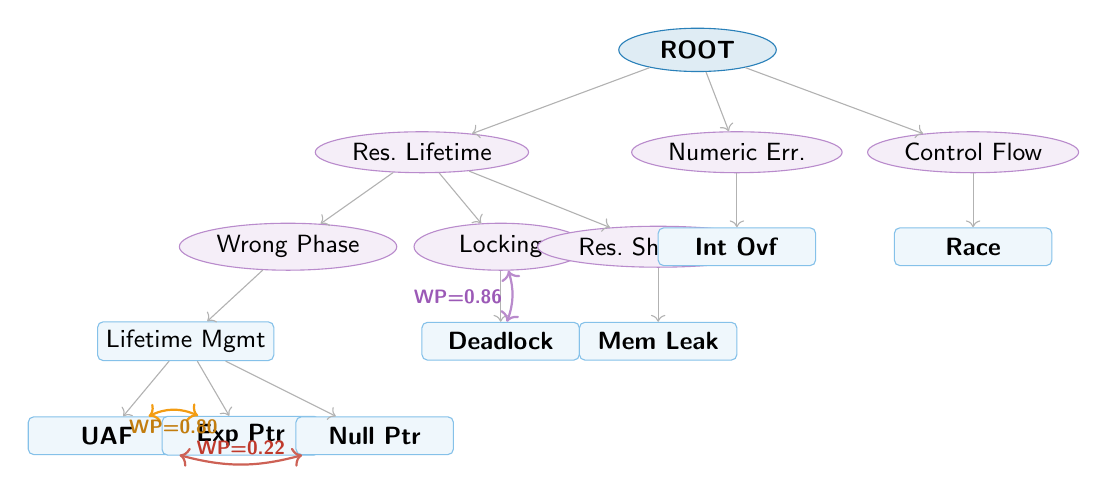
\begin{tikzpicture}[
  root/.style={ellipse,draw=c1,fill=c1!15,font=\small\sffamily\bfseries,
               minimum width=2.0cm,minimum height=0.55cm,inner sep=2pt},
  inter/.style={ellipse,draw=c3!70,fill=c3!10,font=\small\sffamily,
                minimum width=2.2cm,minimum height=0.52cm,inner sep=2pt},
  leaf/.style={rectangle,rounded corners=2pt,draw=c2!60,fill=c2!8,
               font=\small\sffamily,minimum width=2.0cm,minimum height=0.48cm,inner sep=3pt},
  arr/.style={->,gray!60,thin}]

  \node[root] (Nroot) at (0,5.5) {ROOT};

  \node[inter] (N664) at (-3.5,4.2) {Res.\ Lifetime};
  \node[inter] (N682) at (0.5,4.2)  {Numeric Err.};
  \node[inter] (N691) at (3.5,4.2)  {Control Flow};

  \node[inter] (N666) at (-5.2,3.0) {Wrong Phase};
  \node[inter] (N667) at (-2.5,3.0) {Locking};
  \node[inter] (N404) at (-0.5,3.0) {Res.\ Shutdown};

  \node[leaf]  (N672) at (-6.5,1.8) {Lifetime Mgmt};
  \node[leaf]  (N833) at (-2.5,1.8) {\textbf{Deadlock}};
  \node[leaf]  (N401) at (-0.5,1.8) {\textbf{Mem Leak}};
  \node[leaf]  (N190) at (0.5,3.0)  {\textbf{Int Ovf}};
  \node[leaf]  (N362) at (3.5,3.0)  {\textbf{Race}};

  \node[leaf]  (N416) at (-7.5,0.6) {\textbf{UAF}};
  \node[leaf]  (N825) at (-5.8,0.6) {\textbf{Exp Ptr}};
  \node[leaf]  (N476) at (-4.1,0.6) {\textbf{Null Ptr}};

  \draw[arr] (Nroot)--(N664); \draw[arr] (Nroot)--(N682);
  \draw[arr] (Nroot)--(N691);
  \draw[arr] (N664)--(N666); \draw[arr] (N664)--(N667);
  \draw[arr] (N664)--(N404);
  \draw[arr] (N666)--(N672); \draw[arr] (N667)--(N833);
  \draw[arr] (N404)--(N401);
  \draw[arr] (N672)--(N416); \draw[arr] (N672)--(N825);
  \draw[arr] (N672)--(N476);
  \draw[arr] (N682)--(N190); \draw[arr] (N691)--(N362);

  \draw[warn,thick,<->] (N416) to[bend left=25]
    node[below,font=\scriptsize\sffamily\bfseries,warn!80!black] {WP=0.80} (N825);
  \draw[c3!70,thick,<->] (N833) to[bend right=18]
    node[left,font=\scriptsize\sffamily\bfseries,c3] {WP=0.86} (N667);
  \draw[miss!80,thick,<->] (N416) to[bend right=15]
    node[above,font=\scriptsize\sffamily\bfseries,miss] {WP=0.22} (N476);
\end{tikzpicture}

\vspace{0.3em}
{\scriptsize\color{black!55}
Ellipses = intermediate taxonomy nodes.\quad
Rectangles = dataset CWE leaf classes.\quad
Coloured arcs show selected Wu-Palmer scores.}
\end{frame}

% ══════════════════════════════════════════════════════════════════════
\section{Cross-CVE Callgraph}
% ══════════════════════════════════════════════════════════════════════

\begin{frame}{Cross-CVE Callgraph: Idea \& Construction}
\begin{columns}[T]
\begin{column}{0.52\textwidth}

  \textbf{Observation}\\[3pt]
  Patches that fix a \emph{Deadlock} call locking primitives.
  Patches that fix \emph{UAF} call allocation or free functions.
  The callee set of $G_{\text{vuln}}$ carries a class signal
  orthogonal to graph structure.

  \vspace{0.9em}
  \textbf{Construction}\\[3pt]
  Extract CALL nodes from each CVE's $G_{\text{vuln}}$
  (excluding Joern internal operators).
  Pairwise \textbf{Jaccard similarity} over callee name sets:

  $$s_c(A,B) = \frac{|\text{callees}(A) \cap \text{callees}(B)|}{|\text{callees}(A) \cup \text{callees}(B)|}$$

  No re-embedding needed at retrieval time — $O(|\text{callees}|)$.

\end{column}
\begin{column}{0.44\textwidth}
  \textbf{Fused retrieval score}

  \vspace{0.5em}
  \centering
  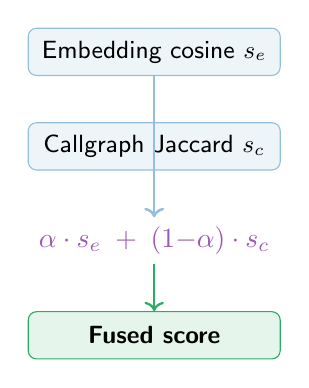
\begin{tikzpicture}[
    box/.style={rounded corners=3pt,draw=c1!50,fill=c1!8,
                minimum width=3.2cm,minimum height=0.6cm,
                font=\small\sffamily,align=center},
    arr/.style={->,thick}]
    \node[box] (emb) at (0,2.2) {Embedding cosine $s_e$};
    \node[box] (cg)  at (0,1.0) {Callgraph Jaccard $s_c$};
    \node[font=\normalsize\sffamily,c3] (pl) at (0,-0.2)
      {$\alpha \cdot s_e \;+\; (1{-}\alpha)\cdot s_c$};
    \node[box,draw=hit,fill=hit!12,font=\small\sffamily\bfseries]
      (fused) at (0,-1.4) {Fused score};
    \draw[arr,c1!50] (emb.south) -- (pl.north);
    \draw[arr,c1!50] (cg.south)  -- (pl.north);
    \draw[arr,hit]   (pl.south)  -- (fused.north);
  \end{tikzpicture}

  \vspace{0.5em}
  {\scriptsize\color{black!55}
  $\alpha=1.0$ = pure embedding baseline.\\
  $\alpha=0.0$ = pure callgraph ranking.\\
  Sweep $\alpha \in [0,1]$ to find the optimal point.}
\end{column}
\end{columns}
\end{frame}

\begin{frame}{Cross-CVE Callgraph: Discriminative Callees}

  \textbf{Top discriminative callees per CWE class}

  \vspace{0.4em}
  {\small
  \renewcommand{\arraystretch}{1.35}
  \begin{tabular}{lp{9.5cm}r}
    \toprule
    \textbf{CWE class} & \textbf{Top callees (high specificity)} & \textbf{Specificity} \\
    \midrule
    Use After Free
      & \texttt{BUILD\_BUG\_ON}, \texttt{read\_pnet}, \texttt{ASSERT\_RTNL}
      & $\geq 0.90$ \\[2pt]
    Deadlock
      & \texttt{queue\_limits\_start\_update}, \texttt{blk\_unfreeze\_release\_lock}
      & $\geq 0.85$ \\[2pt]
    Race Condition
      & \texttt{snd\_pcm\_start\_lock\_irq}, \texttt{snd\_pcm\_drain}
      & $\geq 0.80$ \\[2pt]
    NULL Ptr Deref
      & \texttt{strcmp}, \texttt{intel\_crtc\_for\_pipe}
      & $\geq 0.75$ \\[2pt]
    Integer Overflow
      & \texttt{strncpy}, \texttt{get\_unaligned\_le32}
      & $\geq 0.80$ \\
    \bottomrule
  \end{tabular}}

  \vspace{0.9em}
  \begin{columns}[T]
  \begin{column}{0.48\textwidth}
    \begin{block}{Specificity defined}
      Fraction of all occurrences of that callee that fall within
      this CWE group. Specificity 0.90 means the callee appears
      in UAF patches 90\% of the time.
    \end{block}
  \end{column}
  \begin{column}{0.48\textwidth}
    \begin{block}{Why this works}
      Locking primitives discriminate Deadlock from Race Condition.
      Allocation/free calls separate UAF from Memory Leak.
      Cheap, interpretable, no retraining required.
    \end{block}
  \end{column}
  \end{columns}
\end{frame}

% ══════════════════════════════════════════════════════════════════════
\section{Reranking Results}
% ══════════════════════════════════════════════════════════════════════

\begin{frame}{Knowledge-Augmented Reranking: $\alpha$ Sweep}
\begin{columns}[T]
\begin{column}{0.48\textwidth}

  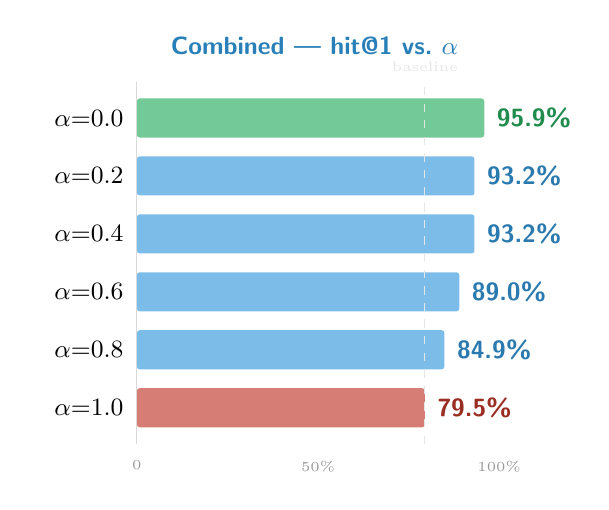
\begin{tikzpicture}[scale=0.92]
    \foreach \y/\alph/\val/\pct/\col in {
      5.8/0.0/0.959/95.9\%/hit,
      5.0/0.2/0.932/93.2\%/c2,
      4.2/0.4/0.932/93.2\%/c2,
      3.4/0.6/0.890/89.0\%/c2,
      2.6/0.8/0.849/84.9\%/c2,
      1.8/1.0/0.795/79.5\%/miss}{
      \node[left,font=\small\sffamily,text width=1.1cm,align=right]
        at (0,\y) {$\alpha{=}\alph$};
      \fill[\col!65,rounded corners=1pt]
        (0.05,\y-0.27) rectangle ({0.05+5.0*\val},\y+0.27);
      \node[right,font=\small\sffamily\bfseries,\col!80!black]
        at ({0.05+5.0*\val+0.04},\y) {\pct};
    }
    \draw[black!15] (0.05,1.3)--(0.05,6.3);
    \draw[black!10,dashed] (0.05+5.0*0.795,1.3)--(0.05+5.0*0.795,6.3)
      node[above,font=\tiny\color{black!40}] {baseline};
    \node[below,font=\tiny\color{black!40}] at (0.05,1.2) {0};
    \node[below,font=\tiny\color{black!40}] at (2.55,1.2) {50\%};
    \node[below,font=\tiny\color{black!40}] at (5.05,1.2) {100\%};
    \node[font=\small\sffamily\bfseries,c1] at (2.5,6.8)
      {Combined — hit@1 vs.\ $\alpha$};
  \end{tikzpicture}

\end{column}
\begin{column}{0.50\textwidth}

  \textbf{All embedders — gain from callgraph fusion}

  \vspace{0.4em}
  {\small
  \renewcommand{\arraystretch}{1.3}
  \begin{tabular}{lccc}
    \toprule
    \textbf{Embedder} & \textbf{Embed only} & \textbf{Best fused} & \textbf{$\Delta$} \\
    \midrule
    \rowcolor{hit!15}
    Combined         & 79.5\% & \textbf{95.9\%} & \textcolor{hit}{+16.4 pp} \\
    CodeBERT pattern & 71.2\% & \textbf{86.3\%} & \textcolor{hit}{+15.1 pp} \\
    VulnPattern      & 52.1\% & \textbf{71.2\%} & \textcolor{hit}{+19.1 pp} \\
    CodeBERT seq     & 75.3\% & \textbf{84.9\%} & \textcolor{hit}{+9.6 pp}  \\
    \bottomrule
  \end{tabular}}

  \vspace{0.8em}
  \begin{alertblock}{Important caveat}
    \small $\alpha{=}0$ = pure callgraph Jaccard.
    Augmented variants share callees almost perfectly with their
    original CVE, making this a near-exact identifier in
    self-retrieval. Held-out performance will be lower.
  \end{alertblock}

\end{column}
\end{columns}
\end{frame}

% ══════════════════════════════════════════════════════════════════════
\section{Ensembles}
% ══════════════════════════════════════════════════════════════════════

\begin{frame}{Embedder Ensembles: Strategies}
\begin{columns}[T]
\begin{column}{0.52\textwidth}

  \textbf{Why ensemble?}\\[3pt]
  The oracle — correct if \emph{any} embedder retrieves at rank 1 —
  reaches 91.8\%, far above any single model (79.5\%).
  Structural and semantic embedders fail on different queries;
  combining them should close part of that gap.

  \vspace{0.9em}
  \textbf{Strategies evaluated}
  \begin{description}[\textbf{Fallback cascade}]
    \item[\textbf{Majority vote}]
      Each embedder votes for its top-1; plurality wins.
    \item[\textbf{Conf.\ weighted}]
      Votes weighted by per-embedder confidence score.
    \item[\textbf{RRF}]
      Reciprocal Rank Fusion across all ranked lists.
    \item[\textbf{Fallback cascade}]
      Try Combined first; defer to CodeBERT seq if
      confidence is below threshold; then CodeBERT pattern.
  \end{description}

\end{column}
\begin{column}{0.44\textwidth}
  \centering
  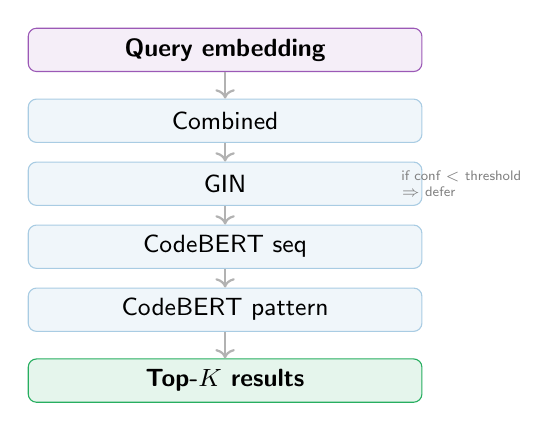
\begin{tikzpicture}[
    box/.style={rounded corners=3pt,draw=c1!40,fill=c1!7,
                minimum width=5.0cm,minimum height=0.55cm,
                font=\small\sffamily,align=center},
    arr/.style={->,thick,black!30},
    note/.style={font=\tiny\sffamily,black!50,align=left}]
    \node[box,draw=c3,fill=c3!10,font=\small\sffamily\bfseries]
      (q) at (0,4.4) {Query embedding};
    \node[box] (e1) at (0,3.5) {Combined};
    \node[box] (e2) at (0,2.7) {GIN};
    \node[box] (e3) at (0,1.9) {CodeBERT seq};
    \node[box] (e4) at (0,1.1) {CodeBERT pattern};
    \draw[arr] (q)--(e1); \draw[arr] (e1)--(e2);
    \draw[arr] (e2)--(e3); \draw[arr] (e3)--(e4);
    \node[note] at (3.0,2.7) {if conf $<$ threshold\\$\Rightarrow$ defer};
    \node[box,draw=hit,fill=hit!12,font=\small\sffamily\bfseries]
      (out) at (0,0.2) {Top-$K$ results};
    \draw[arr] (e4)--(out);
  \end{tikzpicture}
  {\scriptsize\color{black!55} Fallback cascade — each step only fires if the previous confidence is low.}
\end{column}
\end{columns}
\end{frame}

\begin{frame}{Embedder Ensembles: Results}
\begin{columns}[T]
\begin{column}{0.50\textwidth}

  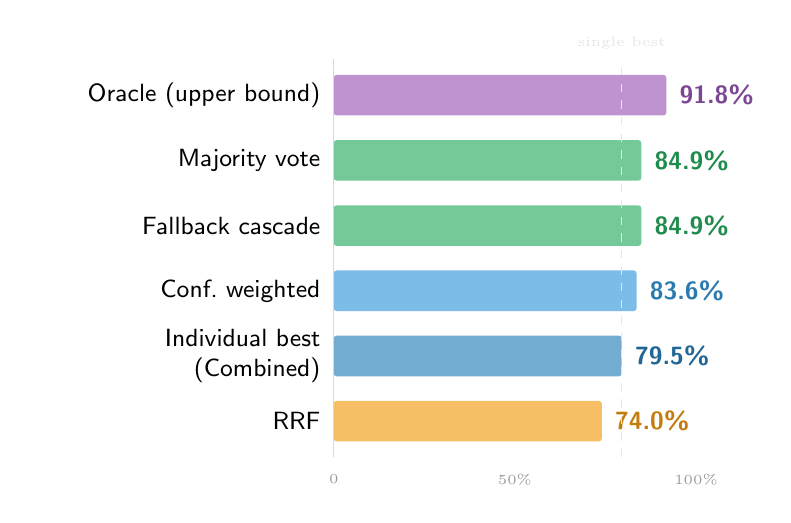
\begin{tikzpicture}[scale=0.92]
    \foreach \y/\lbl/\val/\pct/\col in {
      6.2/{Oracle (upper bound)}/0.918/91.8\%/c3,
      5.3/{Majority vote}/0.849/84.9\%/hit,
      4.4/{Fallback cascade}/0.849/84.9\%/hit,
      3.5/{Conf.\ weighted}/0.836/83.6\%/c2,
      2.6/{Individual best (Combined)}/0.795/79.5\%/c1,
      1.7/{RRF}/0.740/74.0\%/warn}{
      \node[left,font=\small\sffamily,text width=3.6cm,align=right] at (0,\y) {\lbl};
      \fill[\col!65,rounded corners=1pt]
        (0.05,\y-0.28) rectangle ({0.05+5.0*\val},\y+0.28);
      \node[right,font=\small\sffamily\bfseries,\col!80!black]
        at ({0.05+5.0*\val+0.05},\y) {\pct};
    }
    \draw[black!15] (0.05,1.2)--(0.05,6.7);
    \draw[black!10,dashed] (0.05+5.0*0.795,1.2)--(0.05+5.0*0.795,6.7)
      node[above,font=\tiny\color{black!40}] {single best};
    \node[below,font=\tiny\color{black!40}] at (0.05,1.1) {0};
    \node[below,font=\tiny\color{black!40}] at (2.55,1.1) {50\%};
    \node[below,font=\tiny\color{black!40}] at (5.05,1.1) {100\%};
  \end{tikzpicture}

\end{column}
\begin{column}{0.47\textwidth}

  \textbf{Observations}
  \begin{itemize}
    \item Majority vote and cascade both reach \textbf{84.9\%}
          — a \textbf{+5.4 pp} gain over any single model.
    \item RRF \emph{underperforms} the single best (74.0\%) —
          fusing ranked lists dilutes strong individual signals.
    \item Oracle = 91.8\%; the \textbf{7 pp gap} corresponds to
          5 queries that every embedder fails.
          No ensemble strategy closes it.
  \end{itemize}

  \vspace{0.8em}
  \begin{alertblock}{Interpretation}
    \small The 7 pp gap is not recoverable by aggregation.
    It requires a fundamentally different signal —
    either a better graph feature or a held-out-trained model.
  \end{alertblock}

\end{column}
\end{columns}
\end{frame}

% ══════════════════════════════════════════════════════════════════════
\section{Confusion Analysis}
% ══════════════════════════════════════════════════════════════════════

\begin{frame}{Where We Still Fail: Confusion Analysis}
\begin{columns}[T]
\begin{column}{0.50\textwidth}

  \textbf{Top confusions — Combined embedder}\\[4pt]
  {\small 15 misses total; 5 fail every embedder}

  \vspace{0.4em}
  {\small
  \renewcommand{\arraystretch}{1.3}
  \setlength{\tabcolsep}{5pt}
  \begin{tabular}{llcc}
    \toprule
    \textbf{Query CWE} & \textbf{Ret.\ CWE} & \textbf{N} & \textbf{WP} \\
    \midrule
    \rowcolor{miss!15}
    Type Confusion     & Use After Free      & 3 & 0.25 \\
    \rowcolor{miss!15}
    NULL Ptr Deref     & Use After Free      & 2 & 0.22 \\
    NULL Ptr Deref     & Unchecked Return    & 1 & 0.57 \\
    NULL Ptr Deref     & Out-of-bounds Wr.   & 1 & 0.29 \\
    Unchecked Return   & Use After Free      & 1 & 0.25 \\
    \bottomrule
  \end{tabular}}

  \vspace{0.5em}
  {\scriptsize\color{black!55}
  WP $> 0.5$ = taxonomically close (soft miss).\\
  \textcolor{miss!80!black}{Highlighted} rows = taxonomically far — genuine failures.}

\end{column}
\begin{column}{0.47\textwidth}

  \textbf{Why this matters}
  \begin{itemize}
    \item Only 1 of 5 confusion types is taxonomically close
          (NullPtr $\leftrightarrow$ Unchecked Return, WP=0.57).
    \item The dominant error — UAF retrieved for NullPtr or
          Type Confusion — is a \textbf{topological failure}:
          all three patch types add a guard node with
          similar graph structure.
    \item The CWE knowledge graph helps \emph{interpret}
          these errors but cannot fix them.
  \end{itemize}

  \vspace{0.5em}
  \begin{block}{The 5 hard cases}
    \small 5 CVEs fail \emph{every} embedder.
    Hypotheses: trivial single-token patch;
    graph too small; or missing feature
    (pointer aliasing, lock scope, data-flow depth).
    Manual inspection is the next step.
  \end{block}

\end{column}
\end{columns}
\end{frame}

% ══════════════════════════════════════════════════════════════════════
\section{Key Findings}
% ══════════════════════════════════════════════════════════════════════

\begin{frame}{Key Findings}
  \begin{enumerate}
    \item[\faIcon{star}]
      \textbf{Callgraph reranking is highly effective — but verify on held-out data.}\\
      Pure callgraph Jaccard ($\alpha{=}0$) reaches 95.9\% hit@1 for Combined
      (+16.4 pp vs.\ embedding only). However, augmented variants share callees
      nearly perfectly, inflating this number in self-retrieval.

    \vspace{0.7em}
    \item[\faIcon{layer-group}]
      \textbf{Ensembling gains +5.4 pp; oracle reveals a hard 7 pp ceiling.}\\
      Majority vote and cascade reach 84.9\%. The 7 pp gap to oracle (91.8\%)
      corresponds to 5 queries that every embedder fails — not recoverable
      by any aggregation strategy.

    \vspace{0.7em}
    \item[\faIcon{sitemap}]
      \textbf{Confusion errors are topological, not taxonomic.}\\
      Most misses have WP $< 0.4$ — they are genuinely wrong retrievals
      caused by structurally similar patch patterns across different CWE classes.
      The CWE knowledge graph illuminates but does not fix this.

    \vspace{0.7em}
    \item[\faIcon{exclamation-triangle}]
      \textbf{Self-retrieval is a ceiling, not a baseline.}\\
      Numbers are inflated by same-CVE callee overlap in the augmented dataset.
      Held-out evaluation is the prerequisite for all further design choices.
  \end{enumerate}
\end{frame}

% ══════════════════════════════════════════════════════════════════════
\section{Next Steps}
% ══════════════════════════════════════════════════════════════════════

\begin{frame}{Next Steps}
\begin{columns}[T]
\begin{column}{0.60\textwidth}

  \textbf{1. Held-out evaluation (priority)}\\[2pt]
  Build a query set where the correct CVE is not in the index —
  cross-version matches or real bug reports with known ground truth.
  All further architecture decisions depend on this.

  \vspace{0.8em}
  \textbf{2. Inspect the 5 persistent failures}\\[2pt]
  Manually examine the CVEs that fail every embedder.
  Hypotheses: single-token patch; graph too small;
  missing feature (pointer aliasing, lock scope, data-flow depth).

  \vspace{0.8em}
  \textbf{3. Hybrid GIN $\oplus$ CodeBERT embedder}\\[2pt]
  Concatenate GIN (graph topology) with CodeBERT (code semantics)
  and project to 128-d. They fail on complementary queries —
  a fusion should close part of the oracle gap.

  \vspace{0.8em}
  \textbf{4. Semantic graph diff}\\[2pt]
  Replace exact-string $G_{\text{vuln}}$ construction with
  node-level CodeBERT distance thresholding to catch
  logical rewrites invisible to string comparison.

\end{column}
\begin{column}{0.36\textwidth}

  \vspace{0.3em}
  \begin{block}{Current best (self-retrieval)}
    \centering\small
    Callgraph reranked: \textbf{95.9\%} hit@1\\[3pt]
    Ensemble (majority): \textbf{84.9\%} hit@1\\[3pt]
    Oracle upper bound: \textbf{91.8\%}
  \end{block}

  \vspace{0.6em}
  \begin{block}{Target (held-out eval)}
    \centering\small
    Hit@1 $\geq 50\%$ on unseen queries\\[3pt]
    CWE Recall $\geq 60\%$ macro avg
  \end{block}

  \vspace{0.6em}
  \begin{alertblock}{Key risk}
    \small The callgraph gain is partially an artefact
    of same-CVE callee overlap in the augmented dataset.
    Held-out evaluation is the priority.
  \end{alertblock}

\end{column}
\end{columns}
\end{frame}

\begin{frame}[plain]
\centering
\vspace{3em}
{\Large\bfseries\color{c1} Thank you}\\[1.2em]
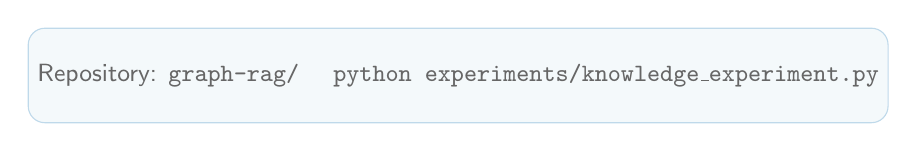
\begin{tikzpicture}
  \node[draw=c1!30,rounded corners=6pt,fill=c1!5,
        minimum width=9cm,minimum height=1.2cm,
        font=\small\sffamily\color{black!60},align=center]
    {Repository: \texttt{graph-rag/} \quad
     \texttt{python experiments/knowledge\_experiment.py}};
\end{tikzpicture}
\end{frame}

\end{document}
